\documentclass[11pt]{article}
% \documentclass[twocolumn]{article}

\usepackage[francais]{babel}
\usepackage[utf8]{inputenc}
\usepackage{enumerate}
\usepackage{amssymb}
\usepackage{amsfonts}
\usepackage{amsthm}
\usepackage{graphicx}
% \usepackage[ruled,vlined,french]{algorithm2e}

% New commands
\newcommand{\xt}{$(X_t)$ }
\newcommand{\om}{$\Omega$ }
\renewcommand\qedsymbol{$\blacksquare$}

% \renewcommand\diffsim{$x \bigtriangleup y$}

% New Environment
\newtheorem{theorem}{Théorème}
\newtheorem{conjecture}{Conjecture}
\newtheorem{propriete}{Propriété}[subsection]
\newtheorem{proposition}{Proposition}[subsection]
\newtheorem{corollaire}{Corollaire}[subsection]
\newtheorem{definition}{Définition}[subsection]
\newtheorem{lemme}{Lemme}[subsection]
\newtheorem{remarque}{Remarque}[subsection]
\newtheorem{claim}{Claim}[subsection]




\begin{document}

\title{Irréductibilité de $X_t$}
\author{Rado Rakotonarivo, Julien David}
\maketitle

\begin{definition}
  On définit par $x \bigtriangleup y$ la \textbf{différence symétrique} entre $x$ et $y$ telle que
  \begin{equation}
    x \bigtriangleup y = \{ u \in x : u \notin y \ \mbox{et} \ v \in y : v \notin x \}
  \end{equation}
\end{definition}

On peut voir la différence symétrique de manière ensembliste comme étant $x \bigtriangleup y = x \cup y \setminus x \cap y$ cependant quelques précisions sont à mentionner:

\begin{itemize}
  \item $x \cup y$ ne constitue pas forcément une enveloppe convexe.
  \item $|x \cup y| = |x| + |y|$ si $x \cap y = \emptyset$.
  \item $x \bigtriangleup y$ est maximal quand $x$ et $y$ n'ont aucun sommet en commun.
\end{itemize}

\begin{lemme}
  Le cardinal de $x \bigtriangleup y$ constitue une borne inférieure de la distance entre $x$ et $y$ dans le graphe de $X_t$, on notera cette distance $\delta(x,y)$ et on a:
  \begin{equation}
    \delta(x,y) \geq{|x \bigtriangleup y|}
  \end{equation}
\end{lemme}

\begin{proof}
  Considérons $x$ et $y \in \Omega$. Comme $x \bigtriangleup y$ constitue l'ensemble des sommets sur lesquels $x$ diffère de $y$ et réciproquement, passer de $x$ en $y$ avec un nombre minimal d'étapes consiste à choisir un chemin qui fera en sorte de réduire $x \bigtriangleup y$ d'un sommet à chaque étape. Par conséquent, il faut au moins $|x \bigtriangleup y|$ étapes pour passer de $x$ en $y$.
\end{proof}

% Pour tout suite d'étapes intermédiaires $(z_i)$ avec $1\leq{i}\leq{\delta(x,y)}$ et $z_i \in \Omega$ on a:
%
% \begin{equation}
%   |x \bigtriangleup y| \geq{|z_i \bigtriangleup y|}
% \end{equation}

\begin{remarque}\label{rmq:difsym}
  Pour passer d'un état $x$ à un état $y$ de $\Omega$, l'idéal serait de directement ajouter des sommets de $y$ et de supprimer ceux de $x$, mais certaines configurations ne le permettent pas. Il faut alors trouver des états transitiores entre $x$ et $y$.
\end{remarque}

\begin{lemme}\label{lem:nb-aretes-simplexe}
  Soit $\mathcal{S}$ un $\mathrm{d}-$simplexe. Le nombre d'arêtes $\nu_\mathcal{S}$ de $\mathcal{S}$ est donné par la relation suivante:

  \begin{equation}
    \nu_\mathcal{S} = \frac{d(d+1)}{2}
  \end{equation}
\end{lemme}

\begin{proof}
  La preuve est immédiate vu que $\nu_\mathcal{S}$ est exactement le nombre de manières de relier deux à deux les $d+1$ sommets de $\mathcal{S}$, i.e. $\nu_\mathcal{S} =$ ${d+1}\choose{2}$ $=\frac{d(d+1)}{2}$.
\end{proof}

\begin{lemme}\label{lem:elim-mauvais-cas}
  Pour tout simplexe $x \in \Omega$ et pour tout $y \in \Omega$. Si on ne peut pas réduire $|x \bigtriangleup y|$ en ajoutant un point dans $y \setminus x$, alors il existe un simplexe $z$, un état transitoire entre $x$ et $y$, avec $\delta(x,z) = 2$ et $|x \bigtriangleup y| = |z \bigtriangleup y|$, tel qu'on peut ajouter un point dans $y \setminus z$ dans le chemin de $z$ vers $y$.
\end{lemme}

\begin{proof}
    Considérons un simplexe $x$ et un état $y$ de $\Omega$ et $\mathcal{H}$ l'hypercube $[0,k]^d$.

    Les seuls cas où l'on ne puisse ajouter aucun point de $y \setminus x$ sont les cas où les éléménts de $y \setminus y$ sont tous des points intérieurs à $Conv(x)$ et/ou des points sur les droites qui supportent les arêtes de $x$. Pour exemple voir le point (1) de la figure \ref{fig:transfo}. Comme on considère le cas de figure où $x$ est un simplexe, ces droites sont au nombre de $\frac{d(d+1)}{2}$ d'après le lemme \ref{lem:nb-aretes-simplexe}.

    Puisque $x$ est un simplexe, la seule transition sortante de $x$ ne peut résulter que d'un ajout de point. L'idée est donc de prouver qu'on peut toujours ajouter un point extérieur à $x \bigtriangleup y$ et d'enlever ensuite un élément de $x \setminus y$. On se retrouverait alors dans un état $z$ qui est un simplexe avec $\delta(x,z) = 2$.

    Deux choses sont à prouver:
    \begin{enumerate}
        \item On peut toujours trouver un point $u$ extérieur à $x \setminus y$
        \item On peut toujours ajouter un point de $z \setminus y$ lors de la transition de $z$ vers $y$
    \end{enumerate}

    \begin{description}
      \item[Claim 1]
      Comme on se trouve dans le cas où l'on ne peut ajouter aucun points de $y \setminus x$, l'idée est de montrer que le nombre de points de $\mathcal{H}$ auquel on a soustrait les points que l'on ne peut ajouter n'est pas nul. En particulier un point nous $u$ suffit.

      Prenons $u$ parmi les sommets de l'hypercube. $\mathcal{H}$ a $2^d$ sommets, au plus $(d+1)$ sommets de $\mathcal{H}$ sont des sommets de $x$ et enfin, au plus $2$ sommets de $\mathcal{H}$ peuvent se trouver sur les $\nu_x$ droites supportant les arêtes de $x$. On pose, $n_a$ le nombre de sommets de $\mathcal{H}$ restants. On a:

      \begin{equation}\label{eqn:sommets-restants}
        n_a \geq{2^d - (d+1) - d(d+1)}
      \end{equation}

      On vérifie que (\ref{eqn:sommets-restants}) est positif non nul dès que $d\geq{6}$. Pour $d<6$, on considère les quantités suivantes:
      \begin{itemize}
        \item $n_h = (k+1)^d$, le nombre de points entiers dans $[0,k]^d$
        \item $n_s$ le nombre de points entiers dans un simplexe, où
        $$
          n_s \leq \left\{
            \begin{array}{rl}
              \frac{(k-1)(k-2)}{2} & \mbox{si } d=2 \\
              \frac{(k+2)(k+1)^{d-1}}{2} & \mbox{si } d\geq{3}
            \end{array}
        $$
        \item $n_c$ le nombre de points entiers sur les droites supportant les arêtes du simplexe, avec:
        $$
          n_c = (k+1) + (d-1)k + {d\choose2}(k-1)
        $$
      \end{itemize}
      Le nombre de points «\textit{non-interdits}» $n_r$ est alors donné par la relation $n_r\geq{n_h - n_s - n_c}$.

    \end{description}





  % Idée de preuves en éliminant les contraintes par symétrie

  % Considérons pour chaque facette $\mathcal{F}_i$ de $x$, le paralellépipède $\mathcal{P}_i$ définit de la manière suivante,
  %
  % \begin{equation}
  %   \mathcal{P}_i = Conv(x \cup \{u_i\})
  % \end{equation}
  % où $u_i$ est le symétrique du sommet $v_i \in X \setminus \mathcal{F}_i$ par rapport à $\mathcal{F}_i$. Le point $u_i$ ici n'est pas forcément entier. Si il ne l'est pas, $\mathcal{P}_i$ n'est pas un état de la chaîne $X_t$.
  %
  % Considérons ensuite l'ensemble $\mathcal{K} = [0,k]^d \cap (\mathcal{P}_i \setminus Conv(x))$ pour tout $i$. Cet ensemble $\mathcal{K}$ est non vide. Supposons que $\mathcal{K}$ soit vide, cela veut dire que pour tou i, les $\mathcal{P}_i \setminus Conv(x)$ sont à l'extérieur de $[0,k]^d$. Or aucun siplexe ne peut recouvrir en entier l'hypercube $[0,k]^d$, par conséquent une partie des $\mathcal{P}_i \setminus Conv(x)$ est contenue dans l'hypercube, i.e. $\mathcal{K}$ est non vide.
  %
  % Comme $\mathcal{K}$ est non vide, le point $u$ extérieur à $x \setminus y$ sera tiré dans $\mathcal{K}$. Voir le point $(2)$ de la figure \ref{fig:transfo}. On pose alors $u = u_1$, on a la transition $z_1 = x \cup \{u_1\}$.
  %
  % La transition suivante va maintenant consister à retirer dans $z_1$ un élément de $x \setminus y$. On retire alors le point $v_i$ de $z_1$ qui correspond au point de $x$ n'appartenant pas à la facette $\mathcal{F}_i$(celle dont on s'en est servi pour la construction de $z_1$) de $x$. On pose alors, $z_2 = z_1 - \{v_1\}$ et on prend $z = z_2$.
  %
  % $LES DROITES \dots$



\end{proof}

\begin{lemme}\label{prop:distance}
  Pour tout $x$ et $y \in \Omega$, $\exists z \in \Omega$, tel que $|x \bigtriangleup y| > |z \bigtriangleup y|$, pour lequel on a $\delta(x,z) \leq{3}$.
\end{lemme}

\begin{proof}
  Considérons $x$ et $y \in \Omega$, tel que $P(x,y) = 0$. Passer de $x$ en $y$ consiste en à trouver un nombre fini d'opérations d'ajouts et de suppressions de sommets; chaque opération correspond à une transition vers un état $z$ qui doit être à priori plus proche de $y$. On observe alors les cas suivants:

  \begin{enumerate}
    \item $x$ est n'est pas un simplexe.
    \begin{enumerate}
      \item $x \subset y$: On ajoute $v \in y \setminus x$ et $z = x \cup \{v\}$, alors $\delta(x,z) = 1$
      \item $x \not\subset y$: On supprime $v \in x \setminus y$ et $z = x - \{v\}$, alors $\delta(x,z) = 1$
    \end{enumerate}
    \item $x$ est un simplexe.
    \begin{enumerate}
      \item Si on peut ajouter $v \in y \setminus x$ alors on le fait, alors $z = x \cup \{v\}$ et $\delta(x,z) = 1$
      \item Sinon:
      \begin{enumerate}
        \item Ajouter un point $u$ extérieur à $x \bigtriangleup y$
        \item Supprimer un élémént de $x \setminus y$
        \item Ajouter un élément de $y \setminus x$

        Dans ce cas on trouve un $z$ tel que $\delta(x,z) = 3$
      \end{enumerate}
    \end{enumerate}
  \end{enumerate}

  D'après le lemme \ref{lem:elim-mauvais-cas}, on peut toujours ajouter un point $u$ extérieur à $x \bigtriangleup y$. Dans tous les cas $\delta(x,z) \leq{3}$. Voir figure \ref{fig:transfo}.



  %Voir le point (1) de la figure \ref{fig:transfo}. Le fait de ne pas pouvoir trouver un état transitoire qui ajoute directement un élément de $y \setminus x$ signifie que tout les éléments de ce dernier sont soit des points intérieurs à $Conv(x)$, soit des points  qui se trouvant sur une droite supportant une arête de $Conv(x)$.

  %La preuve consiste à une construction du chemin entre $x$ et $z$. Le chemin entre $x$ et $z$ est donné par le dernier cas de la remarque \ref{rmq:difsym}, reste à savoir où allons-nous ajouter le point extérieur à $x \bigtriangleup y$.

  %Considérons maintenant pour chaque facette $\mathcal{F}_i$ de $x$, le paralellépipède $\mathcal{P}_i$ = $conv(x \cup \{u\})$ où $u$ est le symétrique du sommet $u_i$ de $x$ n'appartenant pas à $\mathcal{F}_i$, pour tout $1 \leq{i} \leq{d+1}$. On considère également $\mathcal{K} = [0,k]^d \cap (\mathcal{P}_i)_{1\leq{i}\leq{d+1}}$, $\mathcal{K} \neq \emptyset$. On choisit alors un point entier $u \in \mathcal{K}$. On pose $z_1 = x \cup \{u\}$. Voir le point (2) de la figure \ref{fig:transfo}.

  %On retire ensuite de $z_1$ le point $u_1$ n'appartenant pas à la facette $\mathcal{F}_1$ de $x$ utilisée pour la construction de $z_1$. On pose $z_2 = z_1 - \{u_1\}$. Voir le point (3) de la figure \ref{fig:transfo}.

  %Arrivé à cette étape, on remarque que $z_2$ est un simplexe. Nous avons soulevé toutes les difficultés pour avoir une étape transitoire entre $z_2$ et $y$: retrait de $d$ droites supportant les arêtes de $Conv(x)$ et retrait de points intérieurs. Il est maintenant possible d'ajouter un élément de $y \setminus z_2$. On pose alors: $z_3 = z_2 \cup \{v\}$ où $v \in y \setminus z_2$.

  %La transition $z_3 = z_2 \cup \{v\}$ où $v \in y \setminus z_2$ implique que $z_3$ a comme élément un sommet de $y$ de ce fait $|z_3 \bigtriangleup y|<|x \bigtriangleup y|$. En utilisant cette construction on atteint $z_3$ depuis $x$ en au plus 3 étapes i.e. $\delta(x,z_3)\leq{3}$. On prend alors $z = z_3$

  \begin{figure}
    \begin{center}
      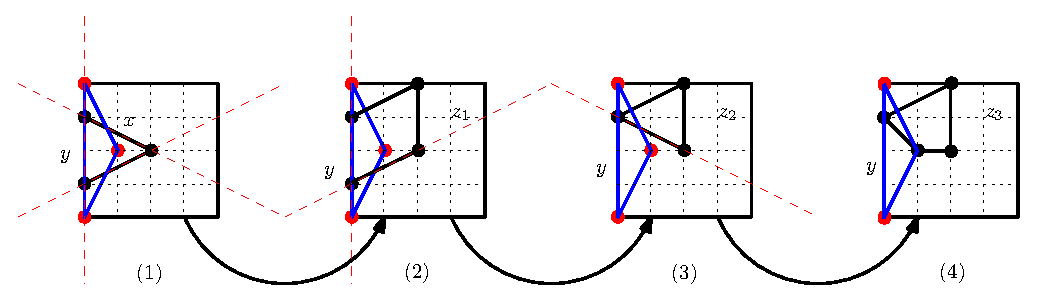
\includegraphics[scale=0.7]{assets/transfo}
      \caption{Ici pour $x$ et $y \in [0,4]^2$, avec $|x \bigtriangleup y| = 6$. On trouve un $z_3 \in \Omega$, tel que $|x \bigtriangleup y| > |z_3 \bigtriangleup y| = 5$, pour lequel on a $\delta(x,z_3) = 3$.}
      \label{fig:transfo}
    \end{center}
  \end{figure}
\end{proof}

\begin{corollaire}\label{cor:diametre}
  Pour tout état $x$ et $y$ de $\Omega$, on a:
  \begin{equation}
    \delta(x,y) \leq{|x| + |y| + 4(d+1)}
  \end{equation}
\end{corollaire}

\begin{proof}
    La preuve est immédiate en applicant le lemme \ref{prop:distance}. Soient $x$ et $y \in \Omega$. Considérons deux simplexes $x^\star$ et $y^\star$ tels que $\delta(x,x^\star) = |x| - (d+1)$, et de même $\delta(y,y^\star) = |y| - (d+1)$. On a la relation suivante:
\begin{equation}
    \delta(x,y) \leq{\delta(x,x^\star) + \delta(x^\star,y^\star) + \delta(y,y^\star)}
\end{equation}
Comme $x^\star$ est un simplexe, au plus il faudra $3(|x^\star| + |y^\star|) = 3 \times 2(d+1)$ étapes, à la marche, pour atteindre $y^\star$ en partant de $x^\star$. Par conséquent:
\begin{equation}
    \delta(x,y) \leq{|x| - (d+1) + |y| - (d+1) + 6(d+1)} = |x| + |y| + 4(d+1)
\end{equation}
\end{proof}

\begin{corollaire}
    $X_t$ est une chaîne de Markov irréductible.
\end{corollaire}

\begin{proof}
    L'irréductibilité découle du corollaire \ref{cor:diametre}. En effet, pour prouver l'irréductibilité de $X_t$, il suffit de trouver un $r_0$ tel que pour tout $x$ et $y \in \Omega$ quand $r \geq{r_0}$ alors $P^r(x,y)>0$. On prend alors $r_0 = |x| + |y| + 4(d+1)$.
\end{proof}



% \begin{proposition}\label{prop:prop2}
%   Tout $(d,k)$-polytope peut se réduire à un simplexe de $[0,k]^d$, et de même à partir d'un simplexe de $[0,k]^d$, on peut atteindre $(d,k)$-polytope.
% \end{proposition}
%
% \begin{proof}
%   Deux choses sont à prouver:
%   \begin{enumerate}[i]
%     \item À partir d'un polytope, on peut se réduire à un simplexe.
%
%     Soit $x,y \in \Omega$, avec $|x| = l$ et $|y| = d+1$. On suppose que $y$ n'est pas encore défini mais on sait seulement que sa taille est de $d+1$, on suppose également que $l$ est suffisament grand par rapport à $d+1$. On remarque que $y$ est un simplexe de dimension $d$. Prouver que le polytope $x$ peut se réduire à un simplexe signifie qu'on peut trouver un $r>0$ et un $y$ tel que:
%     \begin{equation}
%       P^r(x,y)>0
%     \end{equation}
%     Considérons maintenant une marche dans $X_t$ tel que $X_0 = x$. Cette marche consiste à choisir à chaque étape la transition qui enlève à $x$ exactement son $i$-ème sommet et s'arrêter quand l'état de la marche est un état de taille $d+1$.
%
%     Soit $z_i \in \Omega$, $z_i$ va correspondre à l'état dans lequel se trouvera la marche après avoir enlevé le $i$-ème sommet de $x$. On a alors la séquence d'états suivante:
%
%     \begin{equation}\label{eq:eq11}
%       \left\{
%       \begin{array}{rl}
%         z_i &= z_{i-1} - \{v_i\} \  \forall i\geq{1}\\
%         z_0 &= x
%       \end{array}
%       \right.
%     \end{equation}
%
%     En déroulant la récurrence en (\ref{eq:eq11}), on a $z_i = x - \{v_1\} - \dots - \{v_i\}$. On remarque que $z_1 = x -\{v_1\}$ si $|x|>d+1$, d'après nos règles de transition cela implique $P(x,z_1)>0$. En répétant à chaque fois cette opération, en procédant de manière itérative sur les $z_i$, on a $P^i(x,z_i)>0$ si $|z_{i-1}|>d+1$. À l'étape $k = l-d-1$ marche atteint $z_k$, avec $|z_k|=d+1$. On choisit alors $r=k=l-d-1$ et $y=z_k$
%
%     \item À partir d'un simplexe, on peut atteindre un polytope.
%
%     On utilise alors un raisonemment analogue en considérant la marche inverse. De plus les règles de transition nous assure que si $P(x,z_1)>0$ alors $P(z_1,x)>0$.
%
%   \end{enumerate}
% \end{proof}

\end{document}
